\chapter{کار‌های مشابه}
\section{مقدمه}
در این فصل هدف ما بررسی کارهای مشابه است تا بتوانیم از آنها در روند بهبود پروژه کمک بگیریم. همچنین با توجه به نتایج و ارزیابی پروژه‌های دیگر می‌توان بستری فراهم کرد تا نتیایج به دست آمده از این پروژه را با دیگر کارهای مشابه مقایسه کرد.
\\
به صورت کلی پروژه‌هایی با هدف کنترل پهپاد با علائم دست در 3 دسته قرار می‌گیرند.
\begin{itemize}
    \item کنترل پهپاد با کمک بینایی ماشین که شامل شبکه‌هایی برای پردازش تصویر است. 
    \item کنترل پهپاد با دستکش‌های سنسور دار از جمله سنسور تشخیص لختی
     \LTRfootnote{IMU}
      که نیازمند سخت‌افزار خاص برای پیدا کردن موقعیت نقاط کلیدی دست است. با استفاده از یک شبکه عصبی و موقعیت این نقاط می‌توان علائم دست را تشخیص داد. مانند پروژه‌های  \cite{yoo2022motion} و \cite{ma2017hand}.
    \item  کنترل پهپاد با کمک دستگاه کنترل‌کننده حرکت جهشی\LTRfootnote{Leap Motion Controller} که با ردیابی دست، ویژگی‌های آن از جمله موقعیت کف دست و انگشتان، جهت دست و انگشتان، طول و عرض انگشتان و موقعیت مفصل و استخوان‌ها را با دقت بالا اندازه‌گیری کرده و با کمک شبکه‌های عصبی علائم دست را تشخیص می‌دهد. پروژه‌های
    \cite{hu2020deep} و \cite{sarkar2016gesture} نمونه‌ای از این نوع پروژه‌ها هستند. 
\end{itemize}

از بین این موارد این پروژه همانند اولین مورد است که تنها سخت‌افزار مورد نیاز پهپاد, دوربین نصب شده بر روی آن است. 
پروژه‌های مشابه با این پروژه که با کمک پردازش تصویر، پهپاد را کنترل می‌‌کنند به سه دسته کلی تفکیک می‌شوند.
این سه دسته عبارتند از:
\begin{enumerate}
    \item استخراج ویژگی‌های تصویر در هر فریم که با توجه به نیاز‌های مسئله می‌تواند متفاوت باشد، و پیش‌بینی علائم دست براساس ویژگی‌های استخراج شده در مرحله قبل.
    \item تشخیص دست\LTRfootnote{Hand Detection}، ‌برای پیدا کردن موقعیت دست در هر فریم تصویر و سپس ورودی پیکسل‌های دست به صورت قرمز, سبز و آبی
    \LTRfootnote{RGB}
    به مدل، و در نهایت کلاس‌بندی علائم دست.
    \item استخراج نقاط کلیدی\LTRfootnote{Key Point}  دست در تصویر و سپس دادن آنها به عنوان ورودی به مدلی مشخص برای کلاس‌بندی و تشخیص علائم دست.
\end{enumerate}

در ادامه این فصل به بررسی مقالات در این سه زمینه و مقالاتی که بر روی پهباد و پیاده‌سازی مدل‌های هوش مصتوعی تمرکز دارند می‌پردازیم.

\section{مقالات مربوط به ویژگی‌های تصویر}
مقالات به‌کار برده شده در این قسمت بر چگونگی تعیین علائم دست با توجه به تصاویر ورودی داده‌شده بر شبکه عصبی تمرکز دارند. برخی از این مقالات چکونگی ارتباط با پهپاد را نیز پوشش می‌دهند، اما نکته قابل بررسی برای ما چگونگی استخراج ویژگی‌های تصویر و استفاده از آنها برای تعیین علائم دست است.


\subsection[مقاله پهپاد‌های کنترل شده با علائم دست به صورت متن باز]{مقاله پهپاد‌های کنترل شده با علائم دست به صورت متن باز\protect\LTRfootnote{Hand Gesture Controlled Drones: An Open Source Library}}
در این پروژه، تمرکز بر پیاده‌سازی یک سیستم کنترل برای هواپیماهای بدون سرنشین با استفاده از حرکات دست است که مشابه رویکرد مورد بحث در مقاله می‌باشد.
هدف اصلی این پروژه استفاده از شبکه‌های عصبی یادگیری عمیق برای تشخیص لحظه‌های حرکات پویای دست برای کنترل پرواز پهپاد 
است. این تشخیص بر اساس ویژگی‌های هار 
\LTRfootnote{Haar}
 که با توجه به سایه‌ها و رنگ‌های درون تصویر تعیین می‌شوند، انجام می‌شود \cite{natarajan2018hand}.

\subsubsection{\protect\textbf{روش‌شناسی}}
در این پروژه، ابتدا از یک شبکه عصبی برای تشخیص موقعیت دست استفاده می‌شود که به عنوان یک ماژول پیش‌پردازش عمل می‌کند و با دقت بالا موقعیت دست را تشخیص می‌دهد. پس از تشخیص 
موقعیت دست، ویژگی‌های هار از تصویر استخراج می‌شوند. روش تشخیص آن‌ها شامل مجموعه‌ای از الگوریتم‌های تشخیص ویژگی هستند که از تصاویر استفاده می‌کنند تا ویژگی‌ها را 
شناسایی کنند. ویژگی‌های هار بر اساس تغییرات گرادیان در تصویر تعیین می‌شوند و به عنوان الگوهای محلی برای تشخیص حرکات دست استفاده می‌شوند. در ادامه، از شبکه‌های عصبی یادگیری 
عمیق برای تشخیص حرکات دست پویا برای کنترل پرواز پهپاد استفاده می‌شود. این شبکه‌ها عملکرد پیچیده‌ای دارند و با استفاده از ویژگی‌های هار به عنوان داده‌ی ورودی آموزش می‌بینند تا حرکات دست را 
تشخیص دهند و بر اساس آنها دستورات برای حرکت پهپاد را تعیین کنند.
\begin{figure}[h]
    \centering
    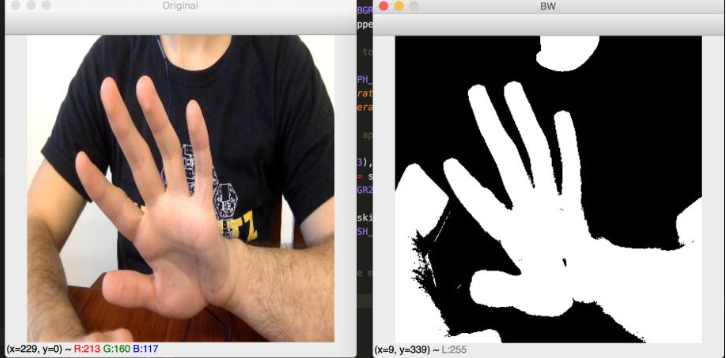
\includegraphics[width=0.7\textwidth]{Haar3.png}
    \caption[ویژگی‌های هار برای استفاده از آستانه رنگ پوست برای تشخیص دست]{ ویژگی‌های هار برای استفاده از آستانه رنگ پوست برای تشخیص دست \cite{natarajan2018hand}}
\end{figure}

این سیستم شامل مراحل پیش‌پردازش داده‌ها، انتخاب ویژگی، ماژول شبکه عصبی برای تشخیص علائم دست و ماژول کنترل پهپاد برای ترجمه 
علائم‌ شناسایی شده به دستورات حرکت پهپاد می‌باشد. علاوه بر این، از مدل ماشین بردار پشتیبان\LTRfootnote{Support Vector Machine} برای کلاس‌بندی و تشخیص حرکات دست استفاده شده است. ماشین بردار پشتیبان به عنوان یک ماشین یادگیری 
 که برای مسائل دسته‌بندی و رگرسیون استفاده می‌شود و در این پروژه برای تشخیص حرکات دست و ترجمه آن‌ها به دستورات حرکت پهپاد مورد استفاده قرار گرفته است. این روش امکان 
کنترل دقیق و پویا برای پهپاد را فراهم می‌کند و از قابلیت‌های پیشرفته یادگیری عمیق برای تشخیص حرکات دست بهره می‌برد.

\begin{figure}[h]
    \centering
    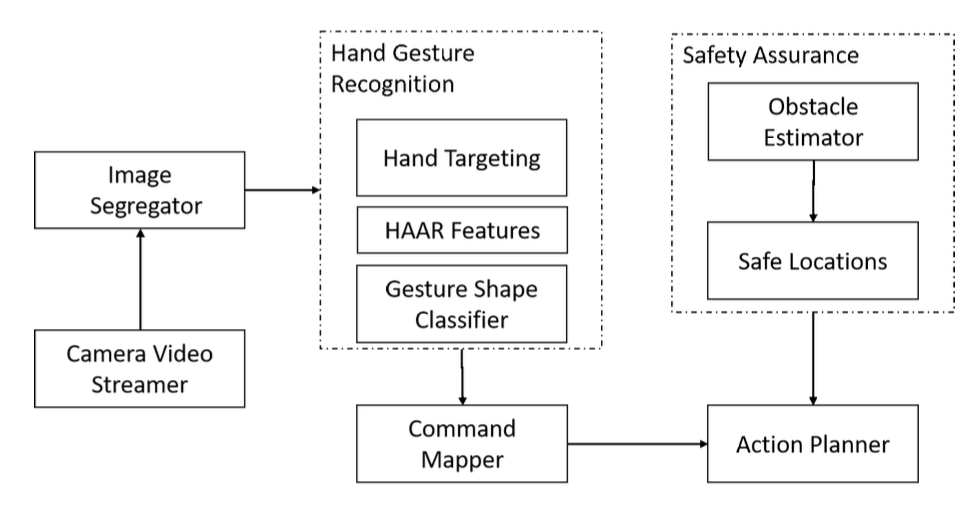
\includegraphics[width=0.8\textwidth]{Haar2.png}
    \caption[چارچوب کنترل پهپاد مبتنی بر علائم دست با کمک ویژگی‌های هار]{چارچوب کنترل پهپاد مبتنی بر علائم دست با کمک ویژگی‌های هار\cite{natarajan2018hand}}
\end{figure}

\subsubsection{\protect\textbf{ نتایج بدست آمده}}
این پروژه دقت بالایی در تشخیص علائم دست و کنترل پرواز پهپاد دارد. پنج حالت دست در این پروژه مدنظر قرار گرفته‌اند و دقت متوسط این مدل، برابر ۴۷۱.۹۷ درصد 
است که نشان‌دهنده عملکرد بسیار عالی آن است. اما لازم به ذکر است که این دقت در پس‌زمینه‌های بهم ریخته و شرایط نوری مختلف 
بسیار متغیر است زیرا ویژگی‌های هار به سایه و رنگ‌های درون تصویر بسیار حساس هستند.



\subsection[مقاله روش‌های تشخیص علائم دست به صورت بی‌درنگ]{مقاله روش‌های تشخیص علائم دست به صورت بی‌درنگ \protect\LTRfootnote{A Real-Time Hand Gesture Recognition Method}}
این مقاله در زمینه پردازش تصویر و تشخیص علائم‌ دست، از روش‌های مبتنی بر مدل‌های ظاهری\LTRfootnote{Appearance Model} به عنوان یک رویکرد موثر استفاده کرده‌‌است.
این روش‌ از ویژگی‌های تصویری و حرکتی دست برای تشخیص و تعیین علائم‌ دست استفاده می‌کند. در این مقاله، روش تشخیص علائم دست به صورت بی‌درنگ و 
قابل اعتماد است که  از تشخیص دست، ردیابی دست\LTRfootnote{Hand Tracking}، تقسیم‌بندی دست\LTRfootnote{Hand Segmentation} و تشخیص ویژگی‌های مقیاس-فضا\LTRfootnote{Scale-Space Feature Detection} برای تشخیص علائم استفاده می‌کند \cite{fang2007real}.

\subsubsection{روش‌شناسی}
در  این مقاله از ترکیب متنوعی از روش‌ها و ویژگی‌های تصویری استفاده می‌شود. این ویژگی‌ها به ترتیب به صورت زیر عمل می‌کنند.
\begin{enumerate}
    \item استفاده از روش آدابوست
    \LTRfootnote{AdaBoost}
    برای تشخیص دست، که یک روش معتبر برای تشخیص اشیاء در تصویر است.
    \item پیگیری دست با استفاده از تشخیص حرکت و رنگ، که از ترکیب تکنیک‌های جریان نوری و نشانه رنگ برای ردیابی دست در تصاویر استفاده می‌شود.
    \item تقسیم‌بندی دست با استفاده از اطلاعات حرکت و رنگ برای تمایز دست از پس‌زمینه و اشیاء دیگر. 
    \item تشخیص ویژگی‌های مقیاس-فضا برای تشخیص علائم دست، که برای شناسایی ساختارهای شبیه به کف دست و انگشتان استفاده می‌شود تا نوع علائم دست توسط ترکیب این ساختارها تعیین شود.
\end{enumerate}
  در نهایت این روش‌ها و ویژگی‌ها با هم ترکیب می‌شوند تا یک سیستم تشخیص دست پایدار و دقیق برای استفاده در رابط کاربری تعاملی و تشخیص علائم دست در زمینه‌های مختلف ارائه شود.

\begin{figure}[h]
    \centering
    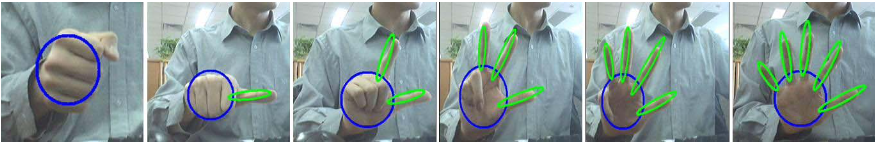
\includegraphics[height=4cm,width=0.9\textwidth]{hand_gesture_feature.png}
    \caption[تشخیص کف دست و انگشتان]{تشخیص کف دست و انگشتان \cite{fang2007real}}
\end{figure}

\subsubsection{نتایج بدست آمده}
اعمال این روش‌ها نتایج قابل قبولی را به همراه داشته است. دقت مدل در تشخیص علائم دست به صورت میانگین 8.93 درصد بوده و از جمله نتایج مهم آزمایشات می‌توان به تشخیص 
صحیح 2436 فریم از کل 2596 فریم ضبط شده اشاره کرد. این نتایج نشان می‌دهند که روش ارائه شده در این مقاله عملکرد قابل قبولی در تشخیص علائم دست دارد و 
می‌تواند به عنوان یک روش موثر برای تعاملات بی‌درنگ استفاده شود.



% \subsection{مقاله \lr{Hand Gesture Recognition using Image Processing and Feature Extraction Techniques}}

% \subsubsection{روش‌شناسی}

% \subsubsection{نتیجه}
% \cite{sharma2020hand}



\section{مقالات مربوط به ورودی تصویر دست به مدل}
مقالات این دسته از جمله پروژه‌هایی هستند که بیشتر از آنکه بر روی پیش پردازش کار کنند باید بر روی معماری خود شبکه تمرکز کنند. در این مقالات تمام یا بخشی از تصویر گرفته شده به صورت یک ماتریس از تصویر با پیکسل‌های متعدد به مدل داده می‌شود. رویکردی که در این نوع پروژه‌ها در پیش گرفته می‌شود، تشخیص موقعیت دست است تا بتوان تنها قسمتی از تصویر را به ورودی شبکه داد که دست در آن وجود دارد تا در حد ممکن
 اندازه ورودی شبکه و دقت آن افزایش یابد. در اینگونه مقالات باید توجه داشت که معماری شبکه را به گونه‌ای برگزید تا در پردازش تصویر بتوان ویژگی‌های مورد نیاز را استخراج کرد.


\subsection[مقاله تشخيص علائم دست برای کنترل پهپاد با استفاده از یادگیری عمیق]{مقاله تشخيص علائم دست برای کنترل پهپاد با استفاده از یادگیری عمیق \protect\LTRfootnote{Hand Gestures For Drone Control Using Deep Learning}}
این پروژه نیز با هدف کنترل پهپاد با استفاده از حرکات دست و شبکه‌های عمیق یادگیری انجام شده است تا بتواند ۹ حالت مختلف دست را شناسایی و به پهپاد، دستور موردنظر کاربر را ارسال کند \cite{hadri2018hand}.

\subsubsection{روش‌شناسی}
در این تحقیق، از معماری شبکه عصبی عمیق \lr{VGG-16} برای تشخیص و تعیین حرکات دست و کنترل پهپاد استفاده شده است. شبکه \lr{VGG-16} یکی از معروف‌ترین و پرکاربردترین شبکه‌های عمیق در زمینه بینایی ماشین است که 
شامل 16 لایه عصبی با لایه‌های پیچشی و ادغام \LTRfootnote{Pooling} می‌باشد. این شبکه برای استخراج ویژگی‌های مهم از تصاویر, استفاده می‌شود. ورودی این شبکه تصاویری است که از دوربین متصل به پهپاد گرفته می‌شود و سپس این 
تصاویر به شبکه وارد می‌شوند. خروجی این شبکه شامل تشخیص حرکات دست مانند حرکات مختلف انگشتان و دست‌ها است. سپس این اطلاعات برای ارسال دستورات کنترلی به پهپاد استفاده می‌شوند. 

\begin{figure}[h]
    \centering
    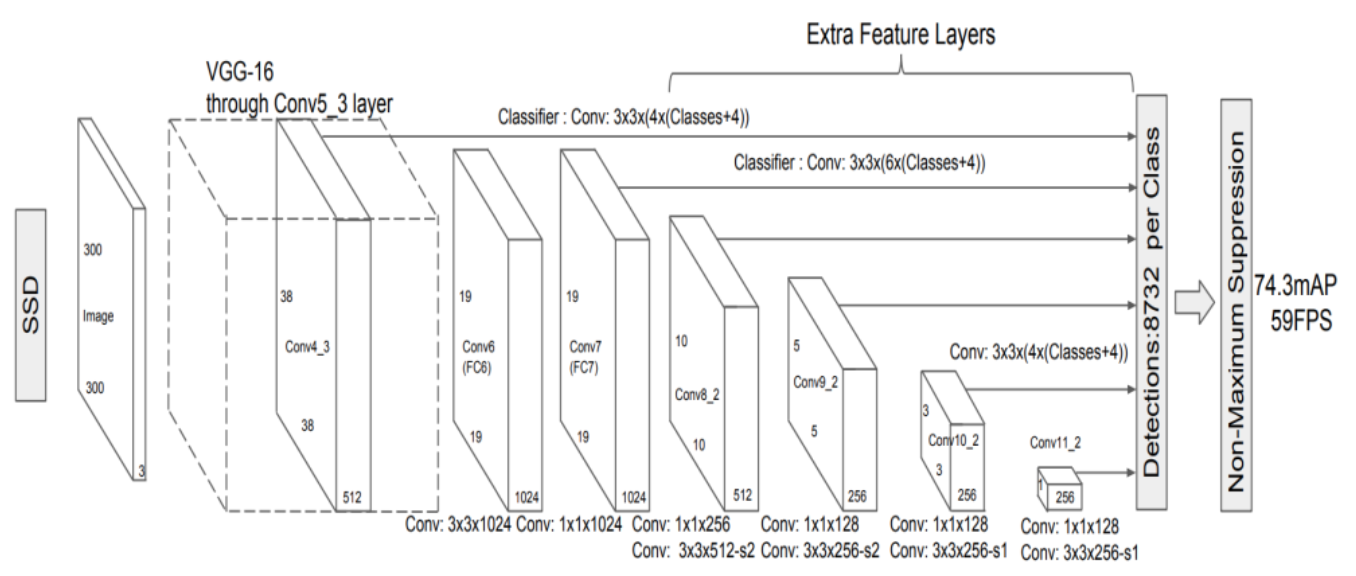
\includegraphics[height=7cm,width=0.9\textwidth]{VGG16.png}
    \caption[معماری \lr{VGG-16}]{معماری \lr{VGG-16}\cite{hadri2018hand}}
\end{figure}

\subsubsection{نتیجه بدست آمده}
 در این پروژه ۹ حالت دست مدنظر قرار گرفته‌شده و دقت آن برابر ۳.۸۳ درصد است.
 که در بهترین حالت ممکن با پس‌زمینه‌ی مناسب بدست آمده و باید در نظر گرفت که این عدد دقت بالایی برای کنترل پهپاد به حساب نمی‌آید.


\subsection[مقاله  علائم یو‌ای‌وی: مجموع‌داده برای یو‌ای‌وی کنترل و تشخيص علائم]{مقاله  علائم یو‌ای‌وی: مجموع‌داده برای یو‌ای‌وی کنترل و تشخيص علائم \protect\LTRfootnote{UAV-GESTURE: A Dataset for UAV Control and Gesture Recognition}}
این مقاله به منظور کنترل پهپاد یا خلبان خودکار با استفاده از حرکت دست پیاده‌سازی شده است. به عنوان مثال، حرکت دست از چپ به راست نشان‌دهنده حرکت پهپاد به راست می‌باشد. 
برای اجرای این برنامه، شبکه \lr{P-CNN} طراحی شده است تا بتواند مفهوم تصاویر را ترجمه کند \cite{perera2018uav}.

\subsubsection{روش‌شناسی}
در این مقاله، از شبکه \lr{P-CNN} \LTRfootnote{Pose-Based Convolutional Neural Network} برای تشخیص حرکات دست استفاده شده است. این شبکه از اطلاعات علائم و حرکت دست و بخش‌هایی از بدن  
استفاده می‌کند. بدین صورت که ابتدا موقعیت دست را با استفاده از جعبه مرزی\LTRfootnote{Bounding Box} مشخص می‌کند و سپس تصویر دست را با استفاده از فیلترهای مناسب وارد شبکه \lr{P-CNN} می‌کند تا بتواند هدف کاربر از حرکت دست را پیش‌بینی کند.
\\
در خروجی این مدل، ۱۳ نوع حرکت مختلف وجود دارد که توسط مدل, مفهوم آنها پیش‌بینی می‌شود. این حرکات شامل کل دست از شانه تا انگشتان و حرکات آنها است. این مدل در پروژه برای دستور دادن به هواپیماهای بزرگ بدون سرنشین در فرودگاه‌ها استفاده می‌شود.
\\
\lr{P-CNN} اطلاعات ظاهر و حرکت را از بخش‌های مختلف بدن استخراج و از دو شبکه پیش‌آموزش داده شده برای محاسبه ویژگی‌های شبکه عصبی پیچشی استفاده می‌کند. در این پروژه برای بخش‌های علائم ظاهری، از شبکه \lr{VGG-f} استفاده می‌شود، و برای 
بخش‌های حرکتی از شبکه \lr{Action Tube} کمک گرفته می‌شود.
در نهایت با ترکیب این دو شبکه با استفاده از روش‌های تجمیع مینیمم و ماکسیمم در هر بعد از تصویر و سپس کنار هم گذاشتن آنها می‌توان حرکت دست را با دقت بالا تشخیص داد.

\subsubsection{نتیجه بدست آمده}
اين مقاله با استفاده از از شبكه \lr{P-CNN} روشي براي كنترل پهپاد با استفاده از حركت و علائم دست پياده‌سازي كرده است. نتايج نشان داده‌اند كه اين روش با دقت ۹.۹۱ درصد، قابليت اجرا در پروژه‌هاي واقعي را دارد.  این پروژه نيازمندي‌هاي پيچيده‌اي براي پياده‌سازي به همراه دارد كه بايد در نظر گرفته شود. این نیاز‌ها شامل سخت‌افزار و نرم‌افزار‌های پیشرفته برای پردازش داده‌های حجیم و پیچیده،
 تنظیمات محیطی مانند نورپردازی و شرایط جوی، تنظیمات دقیق برای تشخیص حرکات و علائم، و مسائل امنیتی مرتبط با کنترل پهپاد است. این چالش‌ها نشان از پیچیدگی‌هایی است که برای اجرای موفق این روش در پروژه‌های واقعی باید در نظر گرفته شوند.




\section{مقالات مربوط به نقاط کلیدی دست}
در این چنین مقالات ورودی شبکه بینایی ماشین برای تشخیص علائم، مختصات نقاط کلیدی دست هستند، که به نوعی یکی از ویژگی‌های تصویر ورودی نیز تلقی می‌شوند. بدین صورت که در ابتدای کار دست کاربر شناسایی شده و سپس نقاط کلیدی آن استخراج می‌شوند تا بتوان حجم داده ورودی به مدل را تا حد امکان کاهش داده و در عین حال داده‌های ورودی را مفیدتر کرد.

% \subsection{مقاله \lr{Hand Gesture Recognition System for Real-Time Application}}
% این مقاله به بررسی سیستم تشخیص حرکات دست در زمان واقعی می‌پردازد. در این سیستم، از الگوریتم \lr{SIFT} برای استخراج ویژگی‌ها از تصاویر
% حرکتی استفاده شده و سپس از مدل \lr{Bag of Feature} و رده‌بند \lr{SVM} برای تشخیص دقیق حرکات دست و دستیابی به عملکرد زمان واقعی استفاده شده است \cite{murugeswari2014hand}.

\subsection[مقاله تشخيص علائم دست برای استفاده‌های بی‌درنگ]{مقاله تشخيص علائم دست برای استفاده‌های بی‌درنگ \protect\LTRfootnote{Hand Gesture Recognition System for Real-Time Application}}
این مقاله به بررسی سیستم تشخیص حرکات دست به صورت بی‌درنگ می‌پردازد. در این سیستم، از الگوریتم سیفت \LTRfootnote{SIFT} برای استخراج ویژگی‌ها از تصاویر حرکتی استفاده شده است. سپس، از مدل دسته‌ای از ویژگی‌ها \LTRfootnote{Bag of Features} و ماشین بردار پشتیبانی برای تشخیص دقیق حرکات دست به صورت بی‌درنگ بهره گرفته‌شده‌ است \cite{murugeswari2014hand}.


\subsubsection{روش‌شناسی}
همان‌طور که گفته‌شد در این مقاله از الگوریتم سیفت  برای استخراج نقاط کلیدی از تصاویر حرکتی دست استفاده شده است. الگوریتم سیفت یک الگوریتم معروف برای استخراج ویژگی‌های برجسته 
و تمایزدهنده از تصاویر است که از مقیاس، جهت و از تغییرات نوری برای استخراج این ویژگی‌ها استفاده می‌کند. این ویژگی‌ها به طور قابل توجهی مستقل از 
مقیاس و جهت تصویر هستند و می‌توانند برای کاربرد‌های گوناگونی از جمله تطبیق قابل اعتماد بین تصاویر مختلف یک شیء مورد استفاده قرار گیرند.

\begin{figure}[h]
    \centering
    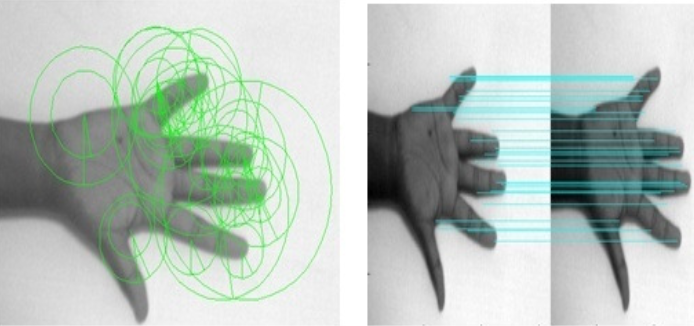
\includegraphics[width=0.5\textwidth]{SIFT.png}
    \caption[تشخیص نقطه کلید و تطبیق توسط سیفت ]{تشخیص نقطه کلید و تطبیق توسط سیفت \cite{murugeswari2014hand}}
\end{figure}

\subsubsection{نتیجه بدست آمده}
الگوریتم سیفت  به عنوان یک ابزار قدرتمند برای استخراج ویژگی‌های برجسته و تمایزدهنده از تصاویر، شناخته شده‌است. این پروژه توانایی تشخیص حرکات دست را با دقت ۸.۹۰ درصد دارد. در این مقاله از روشی نوین و متفاوت برای رسیدن به علائم دست استفاده شده‌است، اما قابل ذکر است که این دقت برای پروژه ما می‌تواند خطای زیادی داشته باشد و در روند پروژه استفاده از این الگوریتم کمک‌کننده نیست.




\subsection[مقاله روش بهبود یافته برای تشخيص علائم دست با استفاده از نقاط کلیدی و جعبه مرزی]{مقاله روش بهبود یافته برای تشخيص علائم دست با استفاده از نقاط کلیدی و جعبه مرزی \protect\LTRfootnote{An Improved Hand Gesture Recognition System Using Keypoints and Hand Bounding Boxes}}
این مقاله یک سیستم بهبود یافته تشخیص حرکات دست با استفاده از نقاط کلیدی و جعبه‌های محدود کننده دست را معرفی می‌کند \cite{dang2022improved}.


\subsubsection{روش‌شناسی}
این پروژه از دو لوله موازی به نام‌های "\lr{MobileNetV2 + FC}" و "\lr{CNN + FC}" تشکیل شده‌است که تصاویر جعبه 
محدود کننده دست و ویژگی‌های استخراج شده از نقاط کلیدی را ترکیب می‌کند و از این طریق علائم دست را پیش‌بینی می‌کند. 
\\
در مدل \lr{MobileNetV2 + FC}، از یک معماری سبک به نام \lr{MobileNetV2} برای استخراج ویژگی‌ها از تصاویر جعبه 
محدود کننده دست استفاده می‌شود. سپس این ویژگی‌ها به یک شبکه عصبی کاملاً متصل
\LTRfootnote{Fully Connected}
(\lr{FC}) داده می‌شوند تا حرکات دست تشخیص داده شوند.
\\
در مدل \lr{CNN + FC} ، در ابتدا نقاط کلیدی دست را که اطلاعات مهمی درباره حرکات دست را شامل می‌شوند پیدا کرده و سپس نقاط به یک شبکه عصبی کاملاً متصل وارد می‌شوند تا حرکات دست
تشخیص داده شوند. این مدل از لایه‌های پیچشی برای کاهش تعداد پارامترها استفاده می‌کند و سپس از لایه‌های کاملاً متصل برای تشخیص حرکات دست استفاده می‌کند.

\begin{figure}[h]
    \centering
    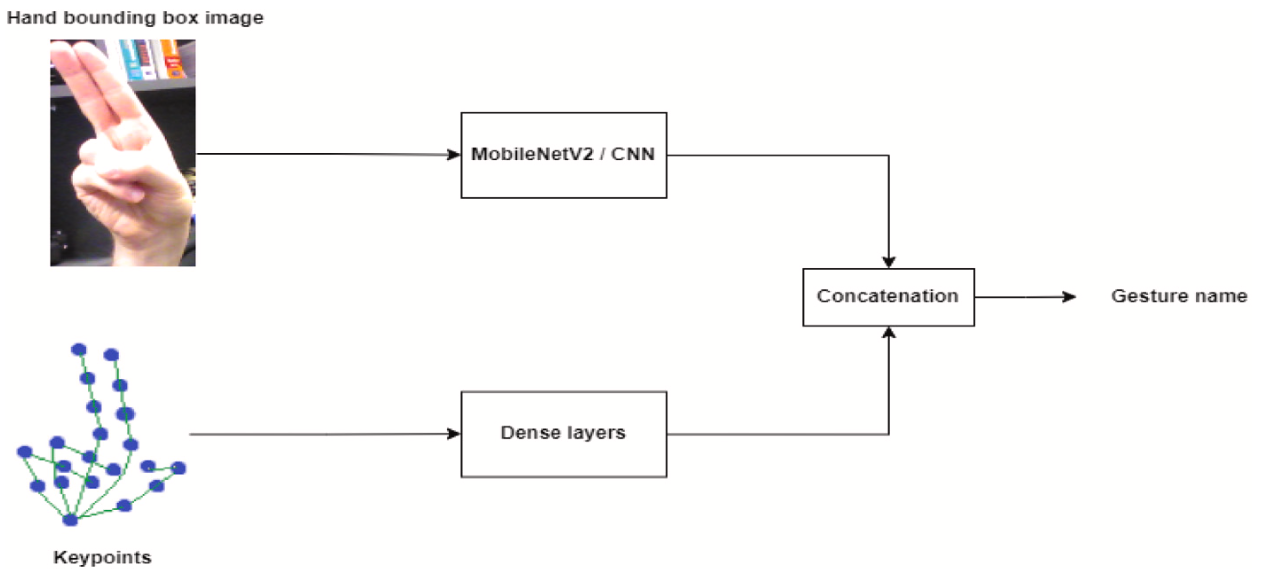
\includegraphics[height=6cm,width=0.8\textwidth]{keypoints_boundingBox.png}
    \caption[معماری ساختار شبکه‌های عصبی دو خط لوله]{معماری ساختار شبکه‌های عصبی دو خط لوله\cite{dang2022improved}}
\end{figure}


\subsubsection{نتیجه بدست آمده}
در صورتی که دو مدل خروجی‌های متفاوتی را پیش‌بینی کنند، از روش‌های ترکیبی مانند ترکیب احتمالاتی استفاده می‌شود تا بهترین تصمیم برای تشخیص علائم دست گرفته شود.
دقت به دست آمده برای تشخیص ۶ علائم دست مختلف در این مقاله در سه مجموع‌داده متفاوت به ترتیب برابر ۹۱، ۹۴ و ۹۶ درصد است.




\subsection[مقاله تشخيص علائم بصری مبتنی بر نقاط کلیدی]{مقاله تشخيص علائم بصری مبتنی بر نقاط کلیدی \protect\LTRfootnote{Visual Gesture Recognition Based On Hand Key Points}}
این مقاله یک روش تشخیص حرکات علائم بصری بر اساس نقاط کلیدی دست ارائه می‌دهد. این روش ابتدا نقاط کلیدی دست را در تصویر ورودی فعلی تشخیص می‌دهد و سپس حرکات تعریف شده را پیش‌بینی می‌کند \cite{chen2021visual}.

\subsubsection{روش‌شناسی}
مدل ارائه شده در این مقاله شامل دو بخش اصلی است: 
\begin{itemize}
    \item مدل تشخیص کف دست که بر اساس ویژگی‌های سخت دست طراحی شده است. برای تشخیص حضور دست در تصویر، از یک مدل \lr{SSD} استفاده شده است که به صورت بی‌درنگ
     تشخیص درست را انجام می‌دهد. و نتیجه آن به صورت یک مستطیل نشان داده می‌شود.
    \item    مدل تشخیص نقاط کلیدی دست که پس از تشخیص حضور دست در تصویر، از این مدل برای تشخیص 21 مختصات نقطه کلیدی دست استفاده می‌شود.  این مدل از الگوریتم نرمال‌سازی برای محاسبه مختصات افقی و عمودی هر نقطه 
    دست استفاده می‌کند. یک سیستم مختصات فضایی برای به دست آوردن مختصات عمق هر نقطه دست نسبت به مبدأ مختصات تعیین شده‌است. در نهایت، معنای حرکات در تصویر ورودی بر اساس رابطه مکانی بین مختصات نقاط کلیدی تعیین می‌شود.
     
\end{itemize}


\begin{figure}[h]
    \centering
    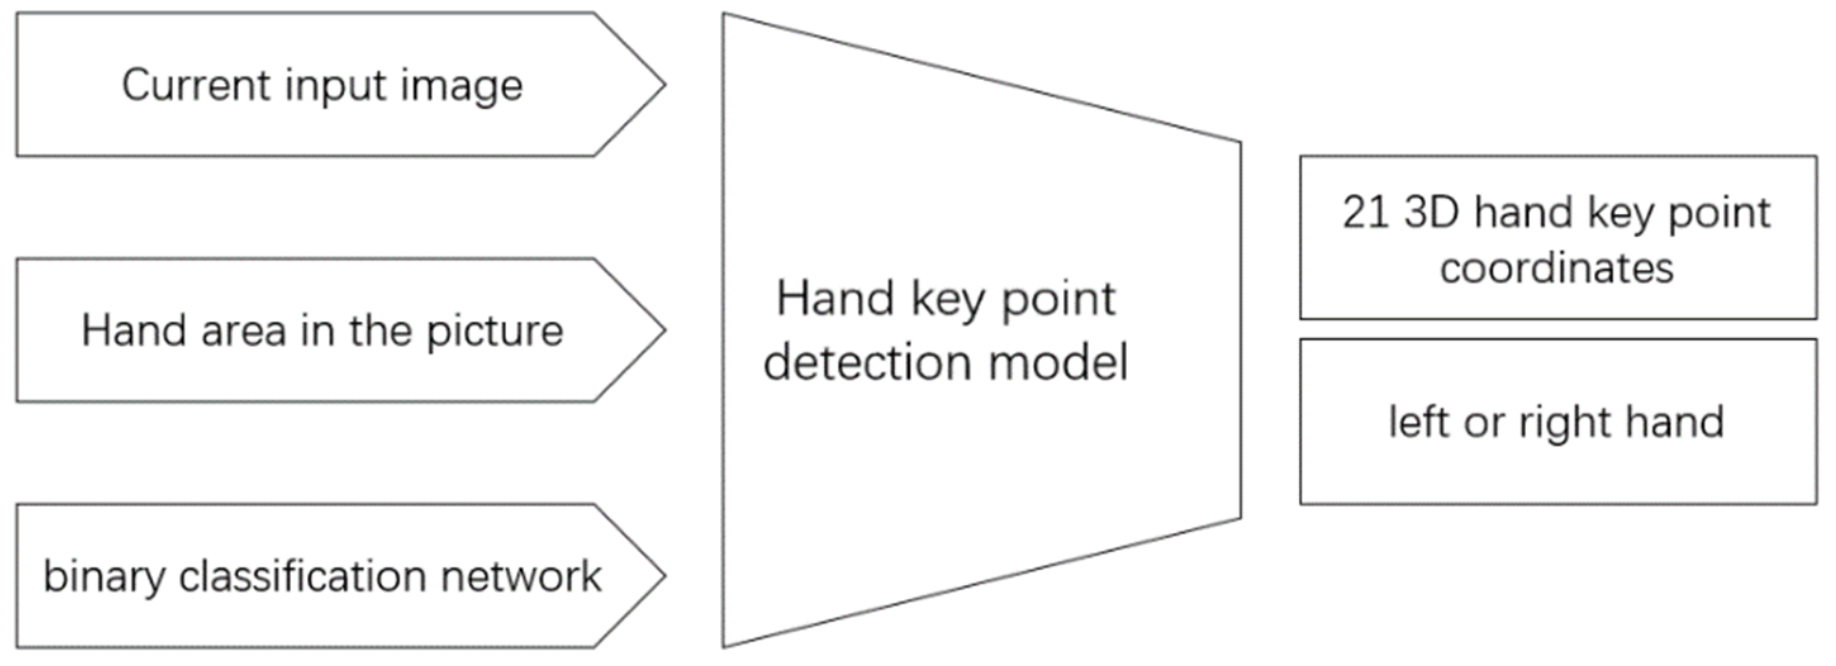
\includegraphics[width=0.7\textwidth]{keypoint.png}
    \caption[ورودی‌ها و خروجی های مدل تشخیص نقاط کلیدی دست]{ورودی‌ها و خروجی های مدل تشخیص نقاط کلیدی دست\cite{chen2021visual}}
\end{figure}

\subsubsection{نتیجه بدست آمده}
این روش دارای دقت بالا و عملکرد مناسبی است. دقت متوسط مدل برابر  ۴.۸۵ درصد تا ۵.۹۸ درصد است که با توجه به جزئیات مدل و پیاده‌سازی پیش‌پردازش می‌تواند انعطاف بالایی داشته باشد در نتیجه می‌تواند راهکار مناسبی تلقی شود.

\pagebreak

\subsection[مقاله دست‌های مدیاپایپ: تشخیص بی‌درنگ دست بر روی دستگاه‌ها]{مقاله دست‌های مدیاپایپ: تشخیص بی‌درنگ دست بر روی دستگاه‌ها \protect\LTRfootnote{MediaPipe Hands: On-Device Real-time Hand Tracking}}
در این مقاله، از کتاب‌خانه مدیا‌پایپ \LTRfootnote{MediaPipe} برای پیش‌بینی ۲۱ نقطه کلیدی دست استفاده‌ ‌شده‌است. این پروژه در موارد گوناگونی از جمله تشخیص علائم دست و افکت‌های واقعیت افزوده \LTRfootnote{Augmented Reality} کاربرد دارد \cite{zhang2020mediapipe}.

\subsubsection{روش‌شناسی}
 برای پیش‌بینی علائم دست  در این پروژه، از دو شبکه  پیچشی استفاده شده‌است. شبکه اول برای پیدا کردن کف دست در تصویر استفاده می‌شود و شبکه دوم ورودی 
موقعیت عکس دست پیدا شده را دریافت و مختصات ۲۱ نقطه عطف را پیدا می‌کند. به کمک این دو شبکه، می‌توان به طور همزمان موقعیت دست‌ها را تشخیص داد و 
نقاط عطف آن‌ها را پیش‌بینی کرد تا برای تشخیص علائم دست در پروژه‌های واقعیت افزوده و واقعیت مجازی استفاده شود.

\subsubsection{نتیجه بدست آمده}
مدل‌های طراحی شده در این مقاله برای تشخیص نقاط عطف دست از دقت ۷.۹۵ درصد برخوردار هستند که دقت بسیار بالایی محسوب می‌شود. این مدل به نور و تصویر پس‌زمینه 
وابسته نیست و دقت متوسط آن در زمینه‌های مختلف اندازه‌گیری شده، لذا این موارد مدل را کاربردی‌تر می‌کند.




\section{مقالات مربوط به آشنایی با پهپاد‌ها و اجرای مدل‌های بینایی ماشین روی آن}
% \subsection{مقاله \lr{Modeling Relation Among Implementing AI-Based drones and Sustainable Construction Project Success}}
% این مقاله با بررسی ارتباط بین استفاده از پهپادهای مبتنی بر هوش مصنوعی می‌پردازد. این تحقیق به بررسی تأثیرات مثبتی که ادغام این دو عنصر می‌تواند در بهبود کارایی و پایداری پروژه‌های
% ساختمانی داشته باشد، می‌پردازد. از آنجایی که استفاده از پهپادها در صنعت ساختمان به سرعت در حال افزایش است و شرکت‌های ساختمانی تحت فشار روزافزونی برای اتخاذ 
% تکنیک‌های بیشتر پایدار و کارآمد قرار دارند، شناخت دقیق‌تری از ارتباط بین موانع و عوامل موفقیت لازم است تا بهترین روش‌ها برای از بین بردن موانع و تضمین موفقیت پهپادها در صنعت مشخص شود \cite{waqar2023modeling}.

\subsection[مقاله مدل‌سازی ارتباط میان پیاده‌سازی‌های مبتی بر هوش مصنوعی بر روی پهپاد‌ها و پروژه‌های کاربردی و موفق ساخت و ساز]{مقاله مدل‌سازی ارتباط میان پیاده‌سازی‌های مبتی بر هوش مصنوعی بر روی پهپاد‌ها و پروژه‌های کاربردی و موفق ساخت و ساز \protect\LTRfootnote{Modeling Relation Among Implementing AI-Based Drones and Sustainable Construction Project Success}}

این مقاله به بررسی ارتباط بین استفاده از پهپادهای مبتنی بر هوش مصنوعی و موفقیت پروژه‌های ساخت‌وساز پایدار می‌پردازد. این تحقیق تأثیرات مثبت ادغام
 این دو عنصر را در بهبود کارایی و پایداری پروژه‌های ساختمانی بررسی می‌کند. با توجه به افزایش سریع استفاده از پهپادها در صنعت، این مقاله به شناخت دقیقی از ارتباط بین این دو از جمله موانع و موفقیت‌ها می‌پردازد. این شناخت به شناسایی بهترین روش‌ها برای از بین بردن موانع و تضمین موفقیت پهپادها در ترکیب هوش مصنوعی کمک می‌کند \cite{waqar2023modeling}.


\subsubsection{روش‌شناسی}
در این تحقیق، از مدل معادلات ساختاری هوشمند برای بررسی موانع و موفقیت اجرای پهپادهای مبتنی بر هوش مصنوعی در صنعت استفاده شده است.
این مدل شامل یک مجموعه جامع از عوامل موفقیت شامل کیفیت، ایمنی و عوامل محیطی است .
\\
پیاده‌سازی مدل‌ها بر روی پهپادها چالش‌هایی ایجاد می‌کند که باید مورد توجه قرار گیرد. این چالش‌ها شامل موارد زیر می‌شود:
\begin{itemize}
    \item پیچیدگی فنی: پیاده‌سازی مدل‌های هوش مصنوعی بر روی پهپادها نیازمند دانش و تخصص فنی بالا است. این امر نیازمند همکاری بین متخصصان مختلف از حوزه‌های مختلف می‌باشد.
    \item محدودیت‌های سخت‌افزاری: پهپادها ممکن است دارای محدودیت‌های سخت‌افزاری مانند ظرفیت پردازشی و حافظه باشند که این محدودیت‌ها موانعی را برای پیاده‌سازی مدل‌های پیچیده ایجاد می‌کنند.
    \item امنیت و حریم خصوصی: استفاده از هوش مصنوعی در پهپادها نیازمند رعایت استانداردهای امنیتی و حفظ حریم خصوصی است. این امر می‌تواند یک چالش مهم برای پیاده‌سازی مدل‌های هوش مصنوعی باشد.
    \item آموزش و توسعه مدل‌ها: پیاده‌سازی مدل‌های هوش مصنوعی بر روی پهپادها نیازمند آموزش و توسعه مدل‌های مناسب برای محیط و وظایف خاص پهپادها است.
\end{itemize}
این چالش‌ها نشان‌دهنده اهمیت اصلی پیاده‌سازی مدل‌های هوش مصنوعی بر روی پهپادها در صنعت است. با غلبه بر این چالش‌ها، می‌توان بهبود 
قابل توجهی در کارایی، ایمنی و پایداری این گونه پروژه‌‌ها داشت.

\subsubsection{نتیجه بدست آمده}
این مقاله نه تنها به شناخت بهتر موانع استفاده از پهپادهای مبتنی بر هوش مصنوعی کمک می‌کند، بلکه راهکارهایی برای غلبه بر این موانع و افزایش موفقیت این تکنولوژی در صنعت ساختمان ارائه می‌دهد. از آنجا که
پهپادها می‌توانند به صورت خودکار و هوشمند وظایف مختلفی را انجام دهند، این تکنولوژی می‌تواند به بهبود مدیریت پروژه، کاهش هزینه‌ها و زمان اجرا، افزایش کیفیت و ایمنی کارها کمک کند.


\subsection[مقاله استفاده از پهپاد دی‌جی‌آی تلو به عنوان پلتفرم تحصیلی در زمینه کنترل مهندسی]{مقاله استفاده از پهپاد دی‌جی‌آی تلو به عنوان پلتفرم تحصیلی در زمینه کنترل مهندسی \protect\LTRfootnote{Use of A DJI Tello Drone as An Educational Platform in the Field of Control Engineering}}
این مقاله یک رویکرد نوآورانه را برای استفاده از پهپاد دی‌جی‌آی تلو \LTRfootnote{DJI Tello} به عنوان یک پلتفرم آموزشی در زمینه مهندسی کنترل ارائه می‌دهد. این مقاله به بررسی نحوه استفاده از ویژگی‌های پهپاد برای 
آموزش مفاهیم کنترل به صورت عملی و جذاب و همچنین چگونگی استفاده از پهپاد دی‌جی‌آی تلو به عنوان یک پلتفرم آموزشی برای مفاهیم کنترل می‌پردازد \cite{ghazi2023use}.

\subsubsection{روش‌شناسی}
در این مقاله، از پهپاد دی‌جی‌آی تلو به عنوان یک ابزار آموزشی و تحقیقاتی استفاده شده است. این پهپاد به دلیل داشتن حسگرهای متنوع و امکان برنامه‌نویسی با زبان برنامه‌نویسی پایتون، به عنوان یک 
ابزار ایده‌آل و انعطاف‌پذیر برای اهداف آموزشی و تحقیقاتی شناخته می‌شود. مقاله به بررسی ارتباط با پهپاد دی‌جی‌آی تلو از طریق زبان برنامه‌نویسی پایتون، امکانات  بسته توسعه نرم‌افزار
\LTRfootnote{Software Development Kit (SDK)}
 رسمی ارائه شده توسط پهپاد، و نحوه ارتباط با پهپاد از طریق وای‌فای و پورت \lr{UDP} می‌پردازد .
\\
در این مقاله، انتخاب پهپاد دی‌جی‌آی تلو برای نمایش مفاهیم ابتدایی مربوط به حوزه کنترل به دلایل گوناگونی انجام شده‌است. از جمله دلایل انتخاب این پهپاد، محبوبیت رو به افزایش آن در بین عموم مردم،
ویژگی‌های چندگانه آن شامل حسگرها، کنترل بازخورد و الگوریتم‌های تخمین برای انجام وظایف پیچیده، و همچنین قیمت مقرون به صرفه آن نسبت به سایر تجهیزات آموزشی است .
\\
برای پیاده‌سازی مدل‌های هوش مصنوعی بر روی پهپاد دی‌جی‌آی تلو، از زبان برنامه‌نویسی پایتون و کتاب‌خانه‌های مختلفی که برای ارتباط با حسگرها و سیستم‌های کنترل پروازی پهپاد ارائه شده استفاده می‌شود. موارد گفته‌شده این 
امکان را می‌دهد که مدل‌های هوش مصنوعی توانایی پیاده‌سازی بر روی پهپاد را داشته باشند و بتوانند عملکرد آن‌ را تحلیل کنند. به عنوان مثال، کاربران می‌توانند از شبکه‌های عصبی یا منطق فازی برای کنترل حرکت پهپاد استفاده کنند.

\begin{figure}[h]
    \centering
    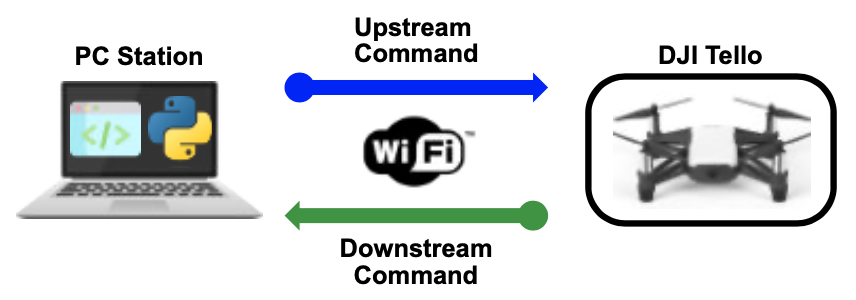
\includegraphics[width=0.8\textwidth]{tello.png}
    \caption[ارتباط برنامه پایتون با پهپاد دی‌جی‌آی تلو ]{ارتباط برنامه پایتون با پهپاد دی‌جی‌آی تلو \cite{ghazi2023use}}
\end{figure}

\subsubsection{نتیجه بدست آمده}
نتیجه این مقاله نشان می‌دهد که استفاده از هوش مصنوعی بر روی پهپاد دی‌جی‌آی تلو عملکرد خوبی را از خود نشان می‌دهد و این ابزار آموزشی و تحقیقاتی می‌تواند به افراد کمک کند تا مفاهیم پیچیده کنترل و هوش مصنوعی را به صورت عملی و جذاب فرا بگیرند. 


\section{جمع‌بندی}

در این فصل به بررسی چهار دسته متفاوت از مقالات پرداخته‌شد 
\begin{itemize}
    \item مقالاتی که با استفاده از استخراج ویژگی‌های تصویر از جمله نور، جهت، موقعیت و ... توانسته‌اند علائم دست را تشخیص دهند. این مقالات برای کلاس‌بندی تعداد علائم محدود و گوناگون از یکدیگر به خوبی عمل می‌کنند، اما در زمانی که تعداد علائم زیاد شده و حالات دست نزدیک به هم باشند، این دقت به صورت چشم‌گیری کاهش پیدا می‌کند. از آنجایی که تمرکز پروژه ما تعیین علائم دست بدون محدودیت تعداد و حالت است این راهکار‌ها عملکرد خوبی را از خود نشان نمی‌دهند.
    \item مقالاتی مربوط به ورودی تصویر دست، نه تنها دقت بالایی از خود نشان نمی‌دهند، بلکه زمان اجرای آنها نسبت به دیگر راهکارها بسیار بیشتر است و می‌تواند پروژه را از بی‌درنگ بودن آن که یکی از بزرگ‌ترین اهداف است دور کند.
    \item مقالات مربوط به تعیین علائم دست با استفاده از نقاط کلیدی عملکرد بسیار خوب و دقت بالایی را از خود نشان داده‌است. این مقالات با توجه به اینکه از چندین مدل پی در پی برای تعیین علائم کمک می‌گیرند از دقت خوبی برخورداند، همچنین حجم پایین این مدل‌ها باعث می‌شود تا بتوان در زمان کوتاهی علائم دست را پیش‌بینی کرد. این مقالات راهکار‌های مناسبی را برای کمک به پیاده‌سازی پروژه ما ارائه دادند.
    \item مقالات مربوط به آشنایی با پهپاد و اجرای مدل‌های بینایی ماشین روی آن دیدگاه جامعی در مورد پهپاد، مشخصات مورد نیاز آن‌ها و چالش‌هایی برای اجرای این پروژه به ما نشان دادند.
\end{itemize}

در تمام مقالات بررسي شده، پروژه‌هایی با هدف تعیین علائم دست به گونه‌اي پياده‌سازي شده‌اند تا حركات را به گونه‌ای كلاس‌بندي كنند كه در خروجي حتما يكي از علائم درنظر گرفته‌شده انتخاب شود. لذا زماني كه دست در حالتي غير از آنها قرار دارد، مدل طراحي شده 
حتما يكي از علائمی را كه به آن شبيه‌تر است انتخاب مي‌كند كه اين امر ميتواند براي پياده‌سازي روي پهپاد واقعي مشكل‌زا باشد و حتي هزينه مالي را به ارمغان آورد. برای پیاده‌سازی پروژه ما باید مسیری را در پیش بگیریم تا بتوانیم این مشکل را برطرف کرده و در عین حال دقت بالایی داشته باشیم.
در فصل بعدی به بررسی دقیق داده‌های استفاده شده در این پروژه‌‌‌, نحوه انجام آن و پیاده‌سازی‌های انجام شده می‌پردازیم.
